\documentclass[a4paper,11pt,twocolumn]{article}
\setlength{\columnsep}{0.5in}
\usepackage{url}
\usepackage[letterpaper,margin=0.75in]{geometry}
\usepackage{times}
\usepackage{graphicx}


\begin{document}

\title{SDN$^{2}$: Marketing System for Datacenter Network Resource Allocation based on Software Defined Network}
\author{Rui Zhou \and Shu Zhang}
\date{Final Project - CSCI 2950-u - Spring 2013}
\maketitle

\begin{abstract}
In this report we present SDN$^{2}$, an auction-based Marketing \emph{S}ystem for \emph{D}atacenter \emph{N}etwork resource Allocation based on \emph{S}oftware \emph{D}efined \emph{N}etworks.
Motivited by similar mechanism of auctions for resource in other computer systems, we aim to 
let users bid their network resouces, mainly bandwidth and latency of their desired flows. Different from existing 
bidding systems like Google's marketing system\cite{google}, our system is based on SDN network and utilizes the advantage
of the central controller and global network information. 
Another thing we focus on is the allocation algorithm for the auctioneer. We investigated some 
algorithms and evaluated their performances. 
\end{abstract}

\section{Introduction}
Resource allocation is an important topic in system related area, especially in data center where network resources heavily influence the performance 
of the applicaton running on the datacenter. Since the network resource is limited and application expense is infinite, an idea of launching auctions on
datacenters for applications to bid resources comes to existence. With the core of auction, other marketing mechanisms have been built for public or 
private datacenters, such as AWS\cite{aws} or internal datacenters for large companies such as Google and Microsoft. While various types of marketing systems
appear, but few of them combine with the existence of SDN network. The appearance of SDN network could provide network manipulators with more powerful 
ways to manage the network. For example, the existence of NIB(Network Informantion Base) in Onix\cite{onix} could provide the upper layer with the global
topology of the entire network just in a single manager machine. 

So in the paper we combine the idea of auction in datacenter networking with the SDN technology so as to reach the goal of bidding network resources. 
Since we have the central information of the network, so bidding and alocations of auctions could be performed in a single node in the network, so as to
reach the goal of real-time allocation. The general work flow is shown in figure 1. 

The general flow of each round of bidding starts from the bidders. Bidders first recognize their flow requirements, for example, they need to buy a flow 
from machine A to machine B in the network with a certain amount of data to transfer, with the hope of minimum bandwidth and latency (QoS) guarantees in 
a certain time period. After confirming these requiremetns, bidders send bidding requests to the auctioneer. The auctioneer collects requests for this 
round and wait for the bidding clock to alert, saying it is time to calculate the allocation. By using specific allocation algorithm, the auctioneer could
get a boolean result for each bidder's request and send the feedback to the bidders, and then a new round starts.

Our goals for this project are, first to build a workable system running the auction and doing allocation in real time, secondly to provision a 
protocol (a standard interface) for all parties wishing to use the system to follow so as to communicate using the protocol, and lastly to investigate
algorithms to allocation resources basing on requests, for different goals. 

In section 2 we investigate some existing datacenter markets and their pricing machanisms. In sections 3 we conclude the contribution of our work. 
In section 4 the design and algorithms of the system are discussed and in the implementation is introduced in sectin 5. In section 6 we do some 
experiments and evaluation on the outcoming products. Since our system is still in the first version, in section 7 we have identified some extensible
work which would be done in the future. And in section 8 we introduce some related work.

\begin{figure}[ht!]
\centering
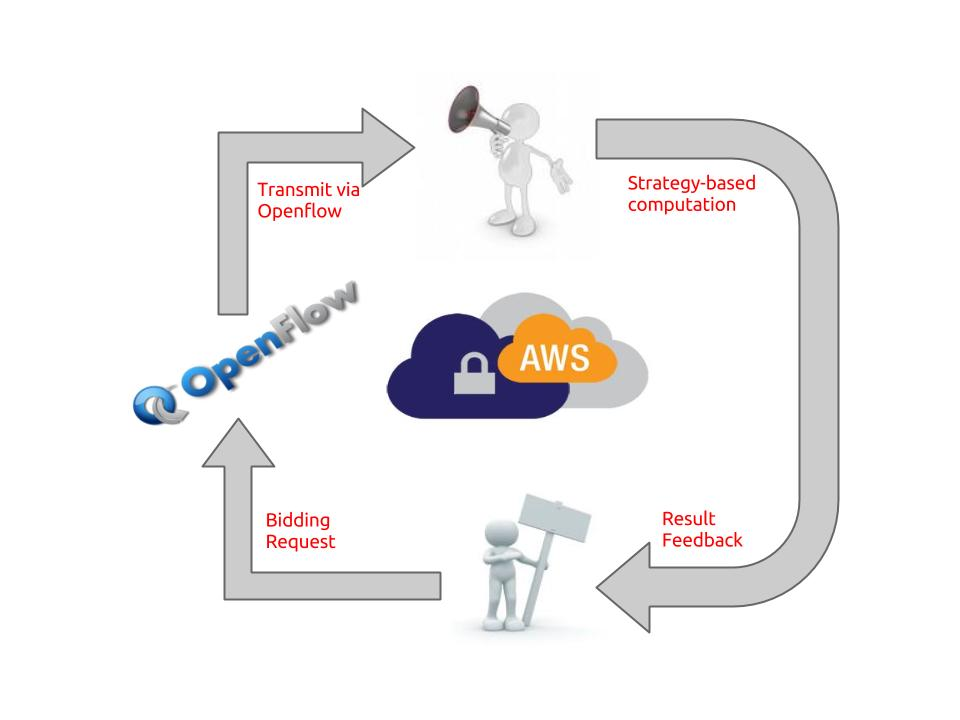
\includegraphics[width=90mm]{general_flow.jpg}
\caption{Auction Working Flow}
\label{overflow}
\end{figure}

\section{Background}
In this section, we investigate exisiting paradigms of data centers (mainly private datacenters and public datacenters) and their marketing and 
pricing methods. Also, we introduce the exisitng techniques of SDN which is the base of our system.
\subsection{Datacenter Markets}
There are generally two types of data centers, one is for-profit, public coud datacenters, such as Amazon Web Services\cite{aws}, the other is private cloud
datacenters, like those operated by Google or Facebook. Although auction machanisms could be applied to both, different scenarios give diverse answers because of 
their business models. The following two paragraphs talks about the assumed behavior for the two types of data centers in this paper and our discussion are 
based upon these behaviors.

In a public cloud service, bidders are customers who use the cloud service. Take Amazon EC2 for example\cite{ec2}, Amazon revises prices for instances for all kinds
of types. Three basic types are On-Demand Instances, Reserved Instances, which allows user to reserve a period of time for future uses and Spot Instances\cite{spot} whose values 
flutuate and allow customers to bid on them. Along this path, Amazon created other services like data transfer, elastic IP addresses, elastic load balancing, etc and 
makes pricing policies for them. From Amazon's view, its pricing policies are so carefully revised so that they could maxmize its profits. If a customer wants to bid for Amazon's 
resources, its knowledge is pretty limited, and Amazon hides the data center details from customers and only expose pricing history as hints for users to bid, and the budget
of buyers are real currency. 

In a private datacenter running inside IT companies, the customers are internal teams of companies who use the datacenter resources for the sake of their team and the companies.
The operator's goal might be minimizing the cost while meeting business objectives, or may be efficient use of network resources. The users (teams), according to their priorities,
are allocated different amounts of budget, which usually is virtual currency. Teams with more budget might use the datacenter resources in a higher share. The private datacenter 
might perform as a autonomy market, whose prices of goods are totally determined by the market or self-adapted by the system. Bidders, with higher possiblity, will be
provided more detailed view of the datacenter conditions, such as dynamic traffic between servers or racks and static network topology, so that they could formulate their 
bidding policies more sensible. 
\subsection{Existing Pricing Mechanisms}
We found that the value of goods which are to be traded in the market is the core issue when letting a market run. People may argue that in an auction,
people could win the bidding by giving the highest amount of money per unit of resource. But sometimes it might be far more complex. Prices, in some cases,
are the reflection of the condition of the market, so it is better to set a baseline price for resources so that people who bid lower than that baseline will
never win the auction, even if they have the highest price. But in some cases, prices do need not to be considered and the simple first-price or second-price auctions
policy could perform well. Also, complex cases like combinatorial pricing\cite{combinatorial auction} is also a must-to-think issue. Also, 
The pricing methods for auctions in private and public datacenters are pretty different. This is because the goals of markets in either datacenters are 
different. 
\subsubsection{Public Cloud Pricing}
Amazon\cite{aws} has set models for pricing in public cloud. AWS supports buy-at-once pricing for on-demand instances as well as auctions for resources
for spot instances. For on-demand services, prices for instances are relatively higher and the good thing is that they are guaranteed to be provided to the buers.
For Spot instances\cite{spot}, Amazon has set the base prices for instances. The prices are much lower (\$0.007 per hour versus \$0.060 per hour for on-demand instances).
The prices are given by Amazon according to their costs and virtual equipments with different capacities will have different prices. Resources
are provided in a combinatorial way, since it is meaningless to bid a single CPU without any memory or storage. But in some scenarios resources are not 
sold in a combinational way, such as Elastic Load Balancing which only charges by the amount of data to be processed by the load balancer.
\subsubsection{Private Cloud Pricing}
Unlike AWS, prices per unit of resources in the private cloud datacenters probably will change in a dynamic way.  Systems like D'Agents\cite{dartmouth} and Google's Planet-wide 
Clusters\cite{google} has adopted dynamic pricing and price of resources are updated periodically. Both the aforementioned systems uses dynamic prices to 
reflect the changing demand-supply relation. For dynamic pricing, the prices are the minimum payment. But in order to maximize the utility of total resources,
the sealed-bid second-price auctions \cite{second price} could be used so as to guarantee that as long as there are more than one bidders in a certain auction round, 
there will always be a winner. The dynamic minimum prices in this case, serve as an indication for bidders to price their bid requests. The prices in \cite{google} could 
change in an self-adaptive way. In short, 'hot' resources will be more expensive and a function (g(x,p)) calculates the price increment after each auction round, basing on the 
exceeding of demands over supplies. Interestingly, AuYoung, et al \cite{ucsd} discovered that auctions might take some time as bidder's patience falls down
when waiting for gaining the resource. So there should be another `buy-it-now' pricing mechanism provided for users who don't want to wait. The buy-it-now
pricing short-circuits the price discovery process of the auction, and the price is determined by a historical function which takes the historical auction/buy-it-now
prices for parameters.


\subsection{Software Defined Network}
\subsubsection{OpenFlow}
OpenFlow is one of the most popular and muture specifications for software defied network curretly existing. It was origianlly propoesed by [] and now is under actively development by the Stanford Opeflow team and a very active cu=ommunity.
OpenFlow primarily defines the control plane of the network. The Novel idea is that one or more cerntral controllers are incharge of setting upp forwarding rules in switches at the granuarity of flows. A flow could be any set of packets that share some particular characteristics,ie,source IP.Packets matching a  flow will be delivered by the switch accordind g to the flow rules, packets brlongs to no flows will be forwarded to switches, The switche then will analyze the packet, determine the forarding rules of this and similar pakcets.
OpenFlow does not reuire major changes to existing switches. Large portios of existing switches ca support OpenFlow with proper firmware updates, and most of the swicth vendors are now adding support for OPenFlow as a standard functionality.
\subsubsection{Floodlight}
With OpenFlow as the foundation, serveral Openflow Controllers were deigned and implmented, including NOX, Nettle and Floodlight. Floodlight was orignally developed by and has become one of most supported and widely used inboth academia and industrial. Flooldlight is written in JAVA. 
Floodlight provides REST APIs for network administrator to take control of the netowrk in the way OpenFlow provides. Meanwhile for developers, floodlight provides a standard way for them to 
add modules into the controller and add workflows. The controller side of SDN$^{2}$ system is implemented via the interfaces and rules Floodlight provides.


\section{CONTRIBUTION}
In this section, we present the contribution of our work.
% what is new ?
%sdn
\subsection{Floodlight and SDN based}
Our work is mounted on Floodlight as its basement. With relatively mutual developed system, Flood light and
our work can be utilized in real world with few set ups.


%fair on user/ flow / 
% resource utilization

\subsection{Fairness and traffic Control }
Bob Briscoe in his paper\cite{bob} has bluntly pointed out that many fairness based on flows are pointless. He argues that
 flows are simply not the right
entities to provide fairness to. We believe in his argument, but it is also arguable that sometimes fairness over flows
can have its usages. Algorithms such as max-min flow generally works well and many people are used to it. In our
work, the total amount of virtual currency/cash  available in our market mechanism resource allocation system at a 
particular time period is proportional to the existing resources available in that  particular period ,by the 
factor of $\alpha$. The total currency/cash is equally distributed to end entities(users or flows) at the beginning of that
 time period. This design will automatically generates fairness among all the users(or flows) and make sure the 
total requests from the users unlikely will  burst too much and exceed the ability of the system. 
The factor $\alpha$ can be 
adjusted over time to reach the best utilization of available resources at each time period. The total traffic 
in  our resource allocation system can be treated as one giant flow with large weight, thus min-max flow can be used
among this  giant flow and others to achieve the maximum usage for all time over the entire system. Weights between users and flows can be 
maintained by adjusting the distribution of virtual cash. Every user has equal amount of virtual cash in a evenly 
weighted system and the properties of strategy-proof and envy free are automatically granted.


%speed -> search
\subsection{Solve by Searching}
Different from allocation for computing resources, the allocation for Network resources requires a much high 
decision speed. In \cite{Sai}, Sai proposed the pattern for agents to keep bidding and potentially face the failure. This works in computation and storage allocation but is
probably not the best strategy in the design of our system. In our work, we had a close look at ideas in logical programming
and tries to seize the best out of it. Our system primarily operates as tree search in a solution space composed
with users' bids are our search are target to optimize a ``profit'' of certain kinds. There isn't much bidding failures
in our system. The amount of virtual cash a bidder spends mainly affect the priority of their resource allocation. 


\subsection{Objective-Oriented Allocation}
Our system supports multiple optimizing modes including : ``Short job first''. ``Maximun profits'', ``best utilization'',
``most met deadlines'' and so on.


\section{System Design and Algorithm}
\subsection{Criteria of the System}
% requirements from five star paper
In [Dominant Resource Fairness: Fair Allocation of Multiple Resource Types], Ali Ghodsi et al'\cite{ali} discussed Dominant Resource Fairness towards 
Fair Allocation of Multiple Resource Types regarding the computation and storage resources. In their discussion several cafeterias
are used to judge one allocation strategy. In this paper, we will adopt the cafeterias but treat the word  word ``cluster'' as ``Network resources'':

\begin{description}

\item 
[Sharing Incentive:]
Each user should be better off
sharing the cluster, than exclusively using her own
partition of the cluster. Consider a cluster with identical nodes and n users. Then a user should not be
able to allocate more tasks in a cluster partition consisting of $\frac{1}{n}$ of all resources.

\item 
[Strategy-proofness:]
Users should not be able to
benefit by lying about their resource demands. This
provides incentive compatibility, as a user cannot
improve her allocation by lying.

\item 
[Envy freeness:]
A user should not prefer the allocation of another user. This property embodies the
notion of fairness [13, 30].

\item 
[Pareto efficiency:]
It should not be possible to increase the allocation of a user without decreasing
the allocation of at least another user. This property is important as it leads to maximizing system
utilization subject to satisfying the other properties.

\end{description}


and In addition  four
other nice-to-have properties:

\begin{description}

\item 
[Single resource fairness:] 
For a single resource, the
solution should reduce to max-min fairness.
\item 
[Bottleneck fairness:]
 If there is one resource that is
percent-wise demanded most of by every user, then
the solution should reduce to max-min fairness for
that resource.
\item 
[Population monotonicity:]
When a user leaves the
system and relinquishes her resources, none of the
allocations of the remaining users should decrease.
\item 
[Resource monotonicity:]
If more resources are added
to the system, none of the.
\end{description}

DRF are able to provide all of the above except for the last \textbf{Resource Monotonicity}.
In fact Ali Ghodsi et al' also gives the follow theorem:
\newtheorem{thm}{Theorem}
\begin{thm}
 No allocation policy that satisfies the sharing incentive and Pareto efficiency properties can also
satisfy resource monotonicity.
\end{thm}

In this paper, we will show that our work can satisfy no less than DRF. In fact, because of the design of our work, several of 
those properties are guaranteed without the need for special care and we can   potentially tackles all of the
properties by in several particular scenarios, which the theorem may not apply due to the design level advantage of our work.

\subsection{Pre-Assumption}
In order to let the system work, we have some pre-assumptions so as to limit the environment. First, we don't specify the unit of 
currency. Although in practice the type of currency should be figured out whether real or artificial, in this system prototype we assumed
the we present money as a LONG type of value. Secondly, we don't care about where and how users gain their money they use to bid. Although in
some existing systems like \cite{ucsd}, all bidders are allocated money at first and then their wealth are adjusted by the bank profit and 
social welfare mechanism, our scenario does not have an `invisible hand` which proforms as a government. Thirdly, our system only works on 
networks with full deployment of SDN networks. Currently the sysetm does not support networks with multiple islands, some of which are 
OpenFlow enabled while others are not. Fourthly, we only constrain users to bid for the machine they reside. 
So if a user in using a machine, he could only bid for flows starting from the using machine. Although supporting
users to bid for other machines are not hard to achieve, we just want to limit the rights the bidders could hold in the network. Another thing 
is that the bidder coud only bid for the future. If it bids for the past, the time will be invalid.
The final major assumption we make is that the working controller never goes down. Since we store 
information in main memory, if the controller crashes, all bidding information maintained in the bidder will be lost, and without the 
replication mechanism it will be a huge problem in our system. For now we temporarily put aside this consideration, and we plan to add
the fail-over mechanism in the future. 



\subsection{Design and Architecture}
In this section we introduce the design and architecture of our system, and also points out our solution to the cafeterias. Also, 
we rule a protocol of exchanging bidding messages which runs in the application layer. There are major two compoenents of the sysetm,
one is running inside the Floodlight controller, which acts as the auctioneer and the other is running on the client machine, 
which performs as a bidding agent for the client. These two sides communicate using the bidding protocol. 

\begin{figure}[ht!]
\centering
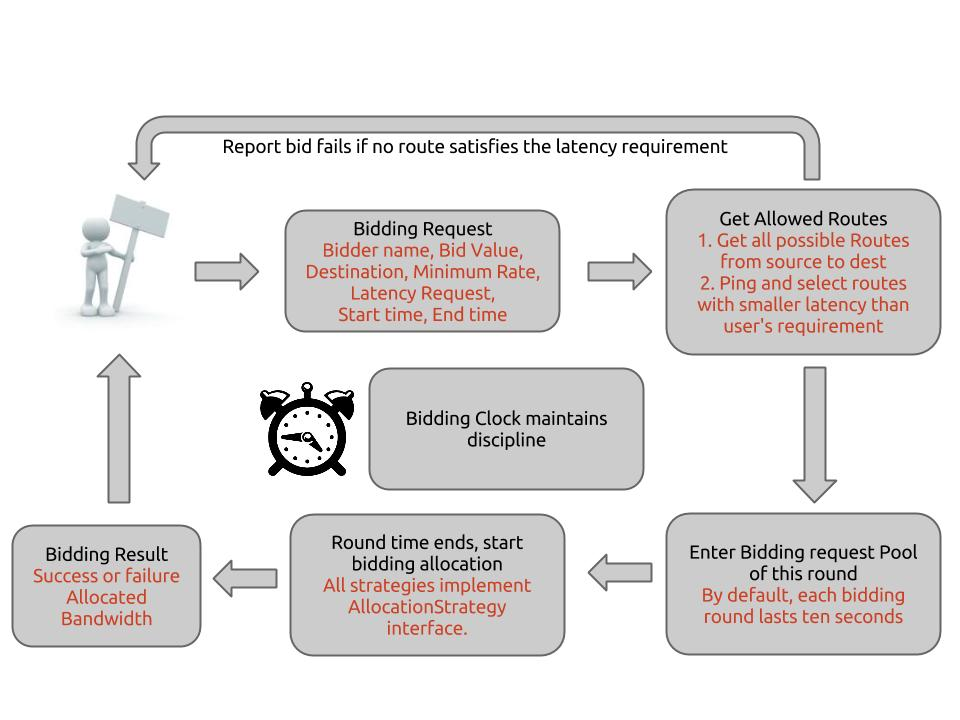
\includegraphics[width=90mm]{flow.jpg}
\caption{Bidder-Auctioneer Interaction}
\label{overflow}
\end{figure}
The interaction between bidders and auctioneers is shown in Figure 2. The bidder sends a bidding request in each round, currently, the 
system needs the user to fill in required fields, including his name, his bidding value, the destination of the flow he wants to bid,
the minimum transform rate he accepts (in the unit of MB/s), the latency he accepts for a packet to 
traval from the source to the destination and the start and end time of the transimission. If 
some fields are what the bidder does not care about, for example the rate, he could just set a special value such as 0 to that field. But 
the start and end time must be set because the computation requires these two fields to be definitely set. Then the bidding request is set 
to the auctioneer aka the bidding manager. Whenever the bidding manager gets a bidding request, it immediately verifies whether the latency
could be satisfied. Because the bidding manager resides in the Floodlight controller with the global topology view of the network, so it could
get all possible routes using the source and destination node. Then for all possible routes, it sends probe packets and count for the time the 
packets use to pass all routes. The administrator could set how many times probe packets are sent for each verification in order to get an 
average real-time latency for the route. If the users' required latency is smaller than the actual probed latency, we just send an bidding 
feedback to the client saying the bid could not be satisfied because of the latency issue. Then for each bidding request, if one of its possible
path could satisfy the latency requirement, these verified routes, along with the original bidding information, are packed together to get into
the bidding request pool, waiting for the bidding round to come. Then for a certain period of time, the auction time arrives, all bidding requests
in the pool are collected and calculated for their results. Then the results are sent to the bidders, which marks the end of the round.

\begin{figure}[ht!]
\centering
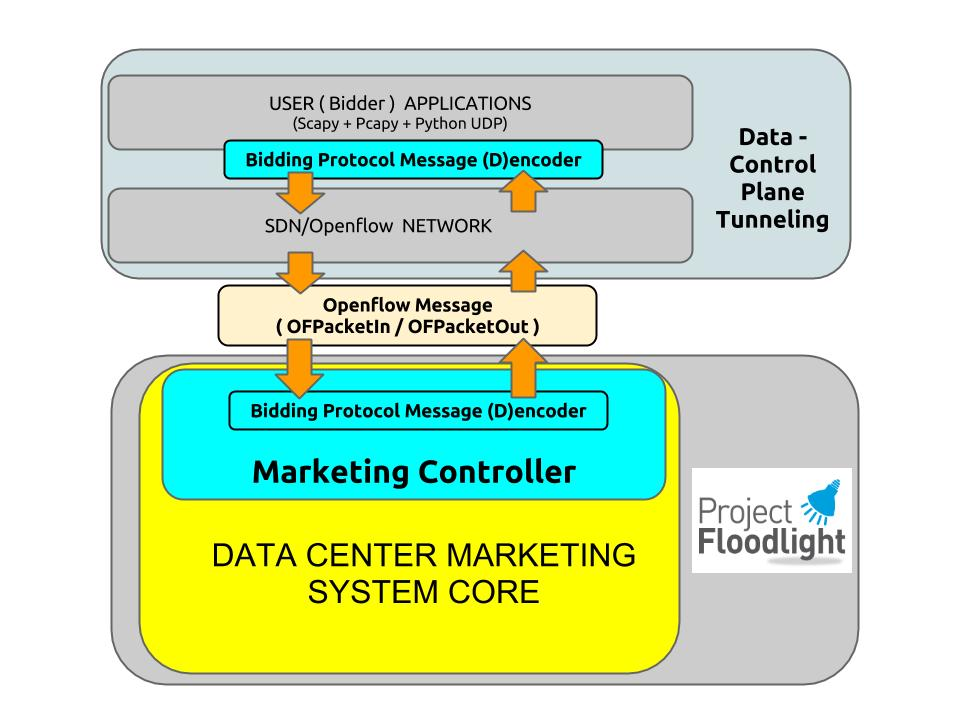
\includegraphics[width=90mm]{architecture_controller.jpg}
\caption{System Architecture}
\label{overflow}
\end{figure}

The system architecture is shown in Figure 3. The user side sends and receives bidding messages formatting in the bidding protocol. These
messages are transmitted via the SDN network. But the packets are in the data plane, and they are destined to the controller which resides
in the control plane, so we utilize the feature of OpenFlow that if the switch does not know the destination IP of a packet or it has not a rule
matching the head of the packet, the swtich will transfer the packet to the controller as a PACKET\_IN message, hence letting the packet go into
the control plane. So the marketing controller is listening the packets as a module of the floodlight framework. If it gets a packet from a 
special IP we make as a mark for the bidding message, the Marketing Controller will decode the message and packet it into a bidding request 
object and pass it to the Marketing Manager which lays in to logic layer, then the Manager could do the thing described in the last paragraph.


\subsubsection{The Biddig Protocol}
There are generally four types of packets we use to pass mesages between bidders and auctioneer. In a typical datacenter, we assume the IP addresses 
are highly clustered and irregular IPs does not appear. So first we assigns speicial IPs for the bidding protocol packets so that either side could 
recoginze the special packets in the data plane. Then we serialize the packet informaiton in JSON. The reason we use JSON is that we want the protocol to
be acoomodated to various machine and data presentation types. 

The bidding request packet is used for the bidders to send their requests to the auctioneer. The bidder name is a String type in Java, and other 
values are all Long (32 bits). Since we only allows users to bid 
for a future period of time, the Start and End time fields in the packet must be positive values and they 
are presented as the relative offset of time comparing with the current time (presented as a long value in the central controller and
we assume the user could know the current time). The speicial source IP for the bidding request packet is 1.2.3.4. The bidding result packet is sent by the auctioneer to the 
bidders. The speicial source IP is 1.2.3.4 and the bidding result is a boolean type and the allowed rate is a allocated rate which must be no smaller than the 
user's requested rate. The latency probe packet is used for the controller to probe the real-time latency between two nodes. The source and destination IP
are set by the controller as the real IP of the two nodes (before sending the latency probe packets, the controller should establish rules on all
switches on the path, using the two IP as matching fields, the out port for the last swtich is 6632 which directs the packet back to the controller).
The Send Reminder Packet is used for reminding bidders to send their flows when their winning bidding time comes. The speicial source IP is 1.2.3.5. The 
packet tells the controller where is the destination of the flow and the duration of this transmission. The reminding mechanism is facilited by the 
timers so that the bidders don't need to record what they have won. The Marketing Manager records these information for the bidder and when the start time 
of their winning bids arrives, the reminder packet is sent.

\begin{figure}[ht!]
\centering
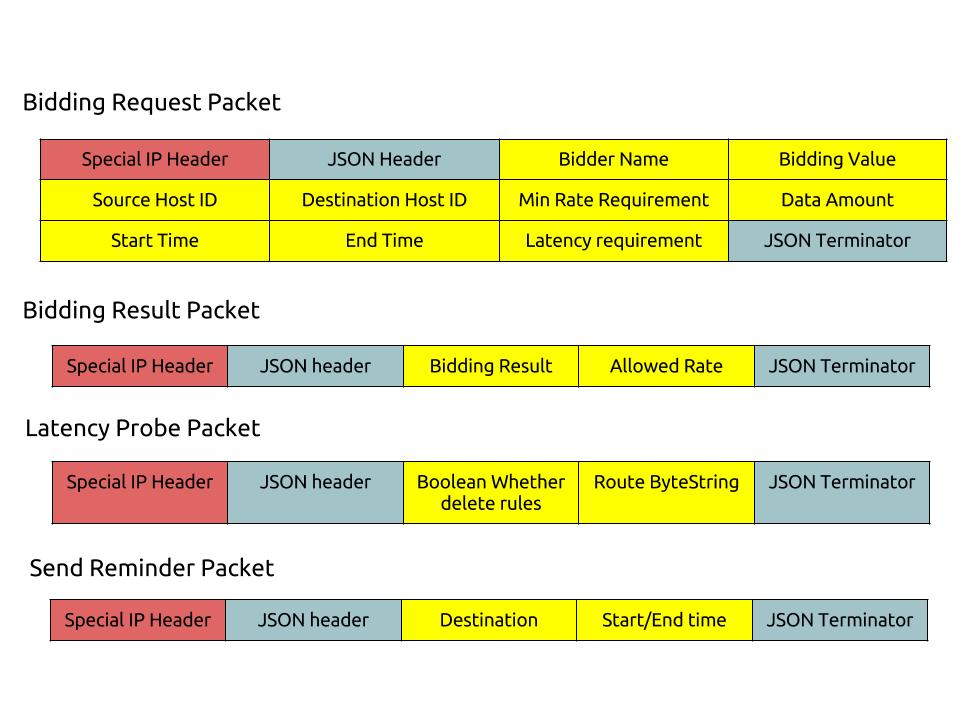
\includegraphics[width=90mm]{protocol.jpg}
\caption{The bidding protocol}
\label{overflow}
\end{figure}

\subsubsection{Marketing Manager}

\begin{figure}[ht!]
\centering
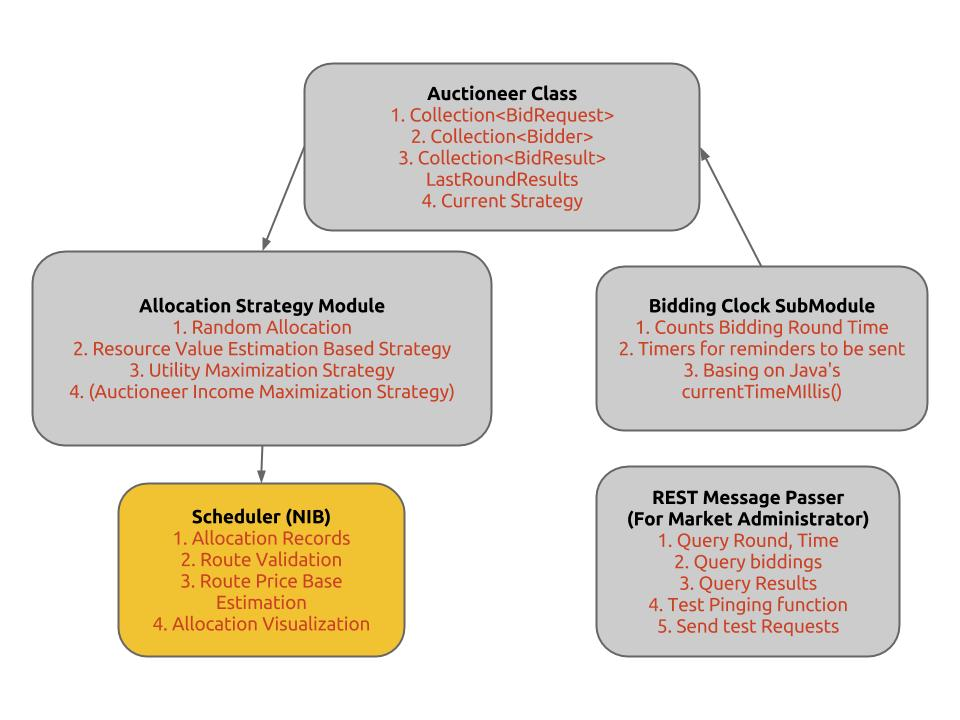
\includegraphics[width=90mm]{core.jpg}
\caption{The Marketing Manager (Auctioneer) Modules}
\label{overflow}
\end{figure}

The internal modules of the Marketing Manager is shown in Figure 4.

\subsubsection{User side bidding agent}



\section{Implementation}


\section{Evaluation}

\section{DISCUSSION AND FUTURE WORK}

Our system is a good starting prototype, the novel idea was there but lots of potential components are remaining to be 
further developed and researched. Some particular interesting potential future work including :

\subsection{Stability Issues}
A significant unsatisfactory we have so far is the stability issue when we test on our Mininet testbed. 
The stability issues happens in multiple forms.  One clear understood common reason the system fails is when the user 
started to bid before the internal controller configure everything it needs. The coming in bidding packet could result in
 exceptions in various place of the system, depending the stage the system is currently within intiliazation phase. 
Besides the obvious easy to fix issues, we sometimes experience random time out of virtual switches simulated by mininet. 
A very common issue is that, floodlight controller would suddenly timeout the netty channel through which a switch is connected, 
due to read time out. Almost instantly after the switch was timed out and disconnected, the controller will detect a new switch 
in mininet, with different real machine port number. This issue happens occasionally, its reason is unknown yet and could resides
 in at least one of floodlight, netty framwork, mininet  or the reference swicth implementation.

\subsection{More Tests and immigrate to real world test bed}
Because of the limit of time and the delay caused by bugs hard to trace(ie, the switch loss bug mentioned aforehead), 
we did not have time to test our system with real switches. It is definitely an item into our todo list and needs to be done in the future.

\subsection{Support of Partial Bidding Request}
In our current settings, users can make request without any requirements on Latency. The user could simply indicate that the latency 
is not important and the bidding agent  could translate as and Long.MAX\_VALUE to put into the request message. However,
 we have not provided a standard when the client only have request for latency but not bandwidth. As a bandwidth of zero make
 no sense regardless of its associated latency, this problem may further redirected to be to help user determine their needs for bandwidth.

\subsection{ Request Translation}
Another very realistic request from users may be the following. 
Most of the users are not able to provide an information detailed enough to assemble a bid request for our system. 
For example, user Bob may only want to download this one Gigabtyte movie tonight so he could watch it tomorrow, 
thus the latency is not so relevant and the shape of his allocation is elastic and dividable. Or 
Alice may want to schedule a phone call  after five minutes and does not really want to specify an end time for it, 
as she does not know in advance. Her request might be composed of an minimun latency, an minimum bandwidth in an extendable session. 
All those real world requests need to be translated by our bidding agent to fits in our bidding system, and our bidding system
 could extend its rules to fit more complex and realistic scenarios. 

\subsection{ Request Predication}
Yet the biggest gap between our system to widely pratical usage is that most of the regular users may not want to make a bid, 
either not able to or no bother to. Thus a great break through that will benefit our system greatly would be enable our bidding
 agent to bid for the users by predicting the potential requests.  Prediction of user requests is solo a much harder problem that 
people are trying to tackle(example ref paper), and its advance could benefit not only our datacenter marketing system but also many 
other existing systems. But as aforementioned, it is generally very hard to achieve in current state of art.



\section{Related Work}
 market is needed in resource allocation,too
Data-centers have rapidly evolved to become the dominating server style in almost
any modern Internet based organizations. As the amount of computation and associated
network  traffic keeps increasing, the needs for efficient and fair  allocation in  Network resources
has also becomes a important topic. There exist enormous number of devices with all 
kinds of different hardware and software among all the data-centers. Different processes and users could
have different requests and requirements. A Hadoop cluster running Map-reduce computations 
may requires great bandwidth.
A web search engine clusters such as Google may want to response to a request 
within a relatively rapid time. All of the needs are to be solved with appropriate network resources
allocation.


% enormous number  of papers have discussed the resource allocation in clusters,
% regarding the computation resource, few on NETwork 
To eliminating possible confusion, allocating \textbf{computing and storage} resources such as Cpus and Memory
 in clusters and date-centers has been a popular topic widely discussed. Researchers have proposed and implemented
various algorithms to achieve fairness and efficiency among different entities. 
%{eaxmple papers} 
Rajkumar Buyya el at' \cite{Rajkumar} proposed architecture for market-oriented allocation of 
resources within Clouds that encompass both customer-driven service management 
and computational risk management to sustain SLA-oriented resource allocation. 
Artur   Czumaj el at'\cite{Artur} proposed  the first thorough theoretical study of the
price of selfish routing in server farms for general cost function, giving the hypothesis that 
distributed entities in data-centers are selfishly motivated.  
Ali Ghodsi el at\cite{Ali} presented fair allocation regarding dominant resources of multiple types
in a data center clusters.
Sai Rahul Reddy P\cite{Sai} in his Master's thesis proposed combined time and budget optimized auction 
algorithms in grid computing. 
However, there exists very few research focusing on the allocation
of \textbf{network} resources. We believe the allocation on \textbf{network} resources such as guaranteed bandwidth and 
jitters are as important as the allocation of computing and memory resources. Computation and storage are not free
thus are entitled to allocation based on market mechanism, so is network resources. This is actually intuitive 
and commonly accepted patterns in real life. Phone carries would sell you a phone for very cheap price and make 
benefits from cellular services, this is a typical example in which the importance of allocation of network resource
 exceed allocation of computation and storage. In data centers, inappropriate abusing of network resources can results
in the failure of the whole system. It has noticed by network administrators that naively running TCP
between hosts can leads to huge overhead on lost packets. Domain specific algorithms like DCTCP\cite{Mohammad} are proposed and applied
in data-centers to effectively avoid collapse and keep traffic moving. But a more agile control was still very hard
to reach due to the distributed nature of inter connected systems, which lacks of a central controller with
a overview for the entire network and the needs of each entities are not really be collected and analyzed to form a strategy. The entire network also do not seek to optimize anything in general.
It would be great if we can have a central view of the network which contact with each participating hosts in the network and allocate resources to them efficiently. Note that
allocation of network resources often requires orders of  magnitude faster than allocation resources in Map-reduce style 
systems due to the fast nature of network transmission.     


% software defined network and participatory network , a central view and participants
While the data-centers technology evolves rapidly, \textbf{Software Defined Network (SDN)} has also been proposed as a
stunning idea. By separating the control panel and the data panel, SDN   abstracts a supported network to be a networking system, which
offers a central view of the networks as a graph and provides a central controller based on flows.
Openflow is a dominating protocol used in SDN based Network systems which defines what is analog to the lower level API in an operating systems.
And high level Networking systems  such as NOX\cite{nox} and Floodlight\cite{floodlight}, and Nettle\cite{nettle} have been developed based on Openflow. SDN and
Network systems has been actively developed in many universities. Companies such as Big Switch and JUNIPER have long 
started to build SDN supported switches. It is believed that the future of network belongs to SDN. in this paper, we also take SDN as the approach towards the effective allocation of Network resources in data-centers. Recently Andrew et al' proposed 	\textbf{Participatory Networking(PNAE)}\cite{andrew}, 
which focuses on the collection of participating entities.  Pane provides serves    analog to the system calls to networking systems, which 
allow the  participating entities to provides hints to network systems and make changes to benefit their needs within allowed privileges.
PANE' structure  nicely forms the base of our allocation mechanism. 

\section{Conclusions}

It should be easy to write your report in LaTeX, and it's a great tool
to learn. It almost certainly came with your Linux installation, and
can be very easily installed in Cygwin and on the Mac (through the
excellent MacTeX distribution).


\section{Acknowledgment}
Thanks Andrew Forguson and Rodrigo Fonseca. Thanks your sisters.

\bibliographystyle{plain}

\begin{thebibliography}{99}
 \bibitem{aws} http://aws.amazon.com.
 \bibitem{floodlight} http://www.projectfloodlight.org/floodlight.
 \bibitem{ec2} http://aws.amazon.com/ec2/pricing.
 \bibitem{spot} http://aws.amazon.com/ec2/spot-instances.
 \bibitem{onix} Koponen, Teemu, et al. "Onix: a distributed control platform for large-scale production networks." Proceedings of the 9th USENIX conference on Operating systems design and implementation. USENIX Association, 2010.
 \bibitem{openflow} McKeown, Nick, et al. "OpenFlow: enabling innovation in campus networks." ACM SIGCOMM Computer Communication Review 38.2 (2008): 69-74.
 \bibitem{google} Stokely, Murray, et al. "Using a market economy to provision compute resources across planet-wide clusters." Parallel \& Distributed Processing, 2009. IPDPS 2009. IEEE International Symposium on. IEEE, 2009.
 \bibitem{combinatorial auction} Nisan, Noam. "Bidding and allocation in combinatorial auctions." Proceedings of the 2nd ACM conference on Electronic commerce. ACM, 2000.
 \bibitem{ucsd} AuYoung, Alvin, et al. Practical market-based resource allocation. University of California, San Diego, 2010.
 \bibitem{dartmouth} Bredin, Jonathan, David Kotz, and Daniela Rus. "Market-based resource control for mobile agents." Proceedings of the second international conference on Autonomous agents. ACM, 1998.
 \bibitem{second price} Vickrey, William. "Counterspeculation, auctions, and competitive sealed tenders." The Journal of finance 16.1 (1961): 8-37.
 \bibitem{clock1} Ausubel, Lawrence M., and Peter Cramton. "Auctioning many divisible goods." Journal of the European Economic Association 2.23 (2004): 480-493.
 \bibitem{clock2} Cramton, Peter, and Lawrence M. Ausubel. "The clock-proxy auction: A practical combinatorial auction design." (2006): 115-138.
 
\end{thebibliography}

\end{document}
